\documentclass[journal]{IEEEtran}
\usepackage{amsmath,amsfonts,amssymb}
\usepackage{graphicx}
\usepackage{booktabs}
\usepackage{microtype}
\usepackage{url}

\title{Supplementary Material: Adversarial Contingency Auctions for Decentralized Multi-Robot Task Allocation under Strategic Blockages}

\author{Kumar~Mrinal$^{1}$%
\thanks{$^{1}$Kumar Mrinal is with the Department of Computer Science and Artificial Intelligence, Indraprastha Institute of Information Technology Delhi (IIIT-Delhi), New Delhi 110020, India (e-mail: {\tt\small mrinal22258@iiitd.ac.in}).}%
}

\begin{document}
\maketitle

\section{Overview}
This supplementary document provides extended statistical visualizations and diagnostics supporting the primary manuscript. All evaluations correspond to the pre-registered benchmark sweep ($N = 250$ matched independent instances, $13,800$ total simulation trials) conducted across 5 graph families, 4 adversary behavioral profiles, and 3 communication regimes.

\section{Extended Performance Distributions}
Fig.~\ref{fig:supp_raincloud} illustrates the full sample distribution across all primary metrics via raincloud plots combining half-violin kernel density estimates, boxplots with interquartile ranges, and jittered instance points.

\begin{figure*}[!t]
\centering
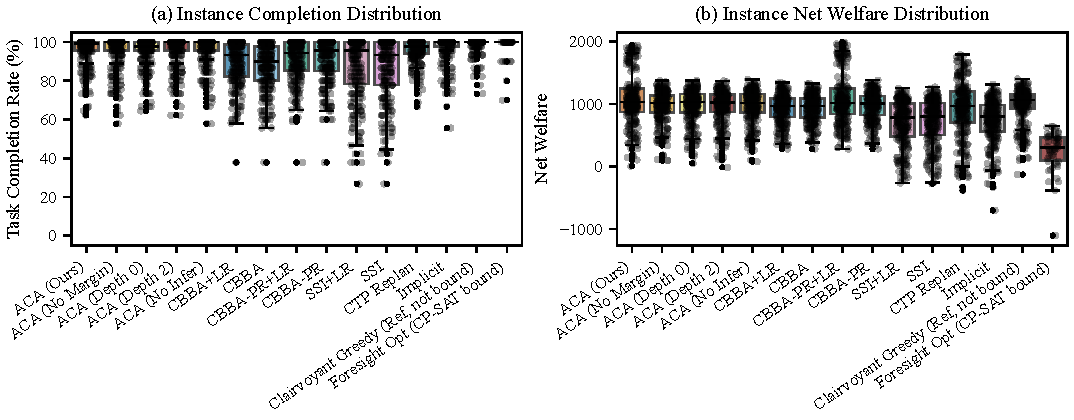
\includegraphics[width=\textwidth,height=7.2cm,keepaspectratio]{static/images/fig_raincloud_performance}
\caption{Raincloud Performance Distributions ($N = 250$ matched instances per method across 5 graph topologies): Panels depict mission completion rate (\%), net team welfare, distinct task conflict counts, and total communication message volume. Boxplots show median and interquartile ranges; half-violins illustrate kernel probability densities; points indicate individual instance evaluations.}
\label{fig:supp_raincloud}
\end{figure*}

\section{Non-Parametric Effect Size Heatmap}
Fig.~\ref{fig:supp_heatmap} details pairwise effect sizes evaluated via Cliff's $\delta$ non-parametric metric across all algorithm pairings.

\begin{figure}[!htbp]
\centering
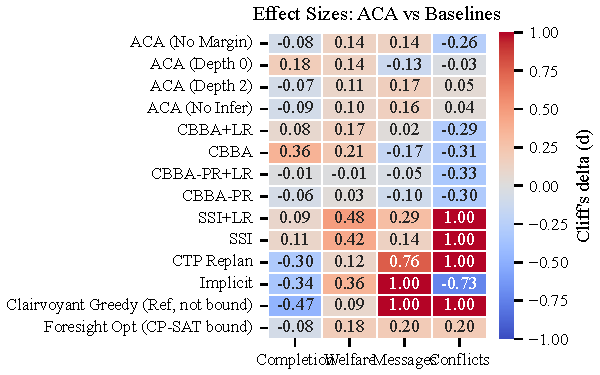
\includegraphics[width=\columnwidth,height=5.5cm,keepaspectratio]{static/images/fig_effect_size_heatmap}
\caption{Pairwise Non-Parametric Effect Size Heatmap (Cliff's $\delta$, $N = 250$ matched instances per comparison): Color gradient indicates magnitude and direction of difference (warm: ACA advantage; cool: baseline advantage). Significance evaluated via Mann--Whitney $U$ test with Holm--Bonferroni correction.}
\label{fig:supp_heatmap}
\end{figure}

\section{Confidence Interval Width Scaling}
Fig.~\ref{fig:supp_ci_scaling} validates statistical sample size adequacy by evaluating empirical 95\% bootstrap confidence interval half-widths as a function of sample instance count $N \in [25, 250]$.

\begin{figure}[!htbp]
\centering
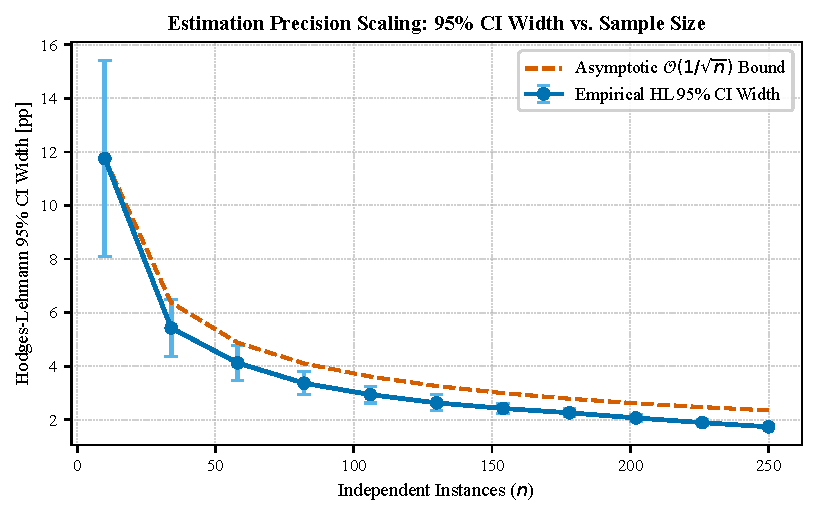
\includegraphics[width=\columnwidth,height=5.2cm,keepaspectratio]{static/images/fig_ci_width_scaling}
\caption{Confidence Interval Width Scaling ($10,000$ bootstrap resamples across subsample sizes $N \in [25, 250]$): Shaded regions depict empirical 95\% bootstrap CI bounds on mission completion rate, demonstrating asymptotic error reduction consistent with $O(1/\sqrt{N})$ central limit convergence.}
\label{fig:supp_ci_scaling}
\end{figure}

\section{Rollout Execution Keyframes}
Fig.~\ref{fig:supp_rollout} provides synchronized execution keyframes on the Downtown Boston road network comparing ACA against CTP Replan and standard CBBA under identical adversarial interdictions.

\begin{figure*}[!t]
\centering
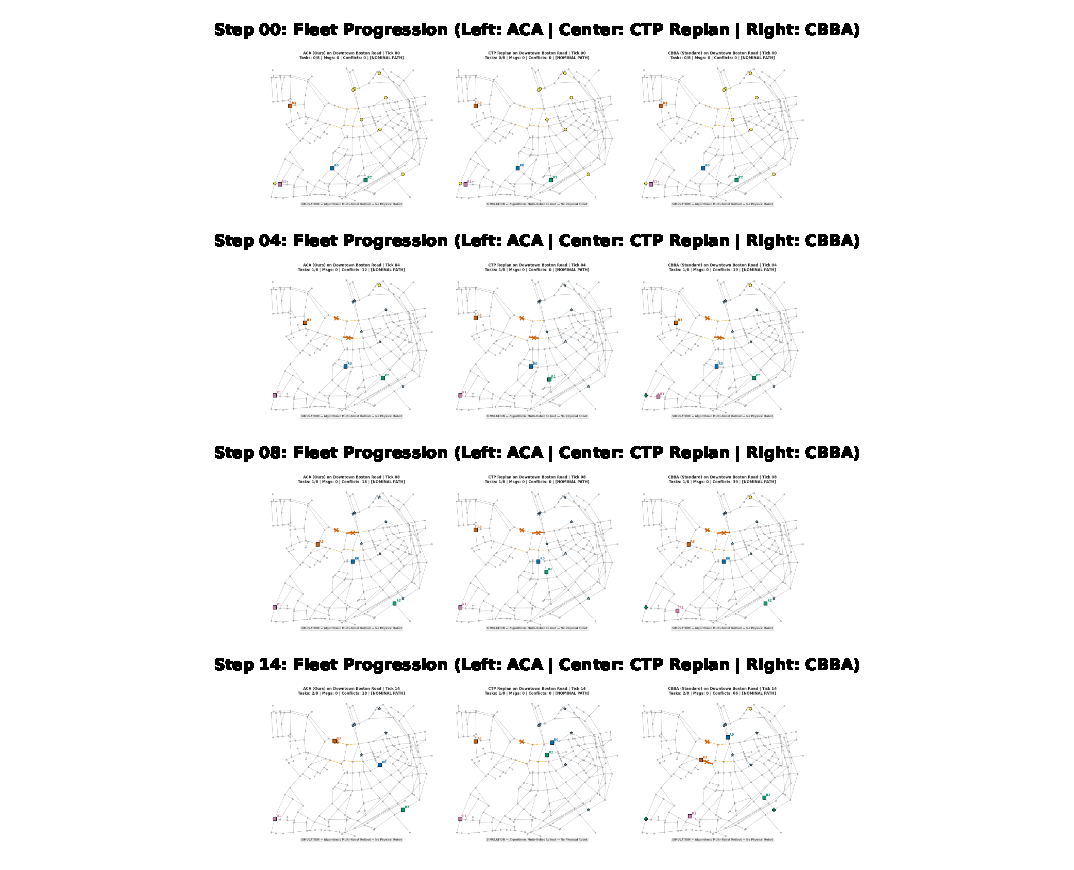
\includegraphics[width=\textwidth,height=5.5cm,keepaspectratio]{static/images/fig_rollout_keyframes_boston}
\caption{Synchronized Rollout Execution Keyframes on Downtown Boston Road Network ($n = 216, |E| = 323$) under Identical Adversarial Blockage Stream: Columns depict ACA (Ours, Left), CTP Replan (Center), and Standard CBBA (Right) across time steps $t \in \{0, 4, 8, 14\}$. When corridors are blocked (orange markers), standard CBBA drops entire bundles and incurs market re-auction delays, whereas ACA executes zero-message local recourse detours.}
\label{fig:supp_rollout}
\end{figure*}

\end{document}
